\documentclass[11pt]{article}
\usepackage[textwidth=18.0cm, textheight=23.0cm, top=2.0cm]{geometry}
\usepackage{pst-all}
\usepackage{amssymb}
\usepackage{tikz}
\usepackage{underscore}\begin{document}
\pagestyle{empty}


ClassName: \underline{\textbf{Class_05.2bp-7}}
\par
BinSize: \underline{\textbf{100 × 100}}
\par
ReduceSize: \underline{\textbf{100 × 100}}
\par
TypeNum: \underline{\textbf{20}}
\par
Num: \underline{\textbf{20}}
\par
OutS: \underline{\textbf{50000}}
\par
InS: \underline{\textbf{40465}}
\par
Rate: \underline{\textbf{0.809}}
\par
UB: \underline{\textbf{5}}
\par
LB0: \underline{\textbf{5}}
\par
LB: \underline{\textbf{5}}
\par
LBWithCut: \underline{\textbf{5}}
\par
NodeCut: \underline{\textbf{0}}
\par
ExtendedNodeCnt: \underline{\textbf{1}}
\par
GenNodeCnt: \underline{\textbf{1}}
\par
PrimalNode: \underline{\textbf{0}}
\par
ColumnCount: \underline{\textbf{5}}
\par
TotalCutCount: \underline{\textbf{0}}
\par
RootCutCount: \underline{\textbf{0}}
\par
LPSolverCnt: \underline{\textbf{1}}
\par
PricingSolverCnt: \underline{\textbf{0}}
\par
BranchAndBoundNum: \underline{\textbf{1}}
\par
isOpt: \underline{\textbf{true}}
\par
TimeOnInitSolution: \underline{\textbf{600.000 s}}
\par
TimeOnPrimal: \underline{\textbf{0.000 s}}
\par
TimeOnPricing: \underline{\textbf{0.000 s}}
\par
TimeOnRmp: \underline{\textbf{0.063 s}}
\par
TotalTime: \underline{\textbf{600.328 s}}
\par
\newpage


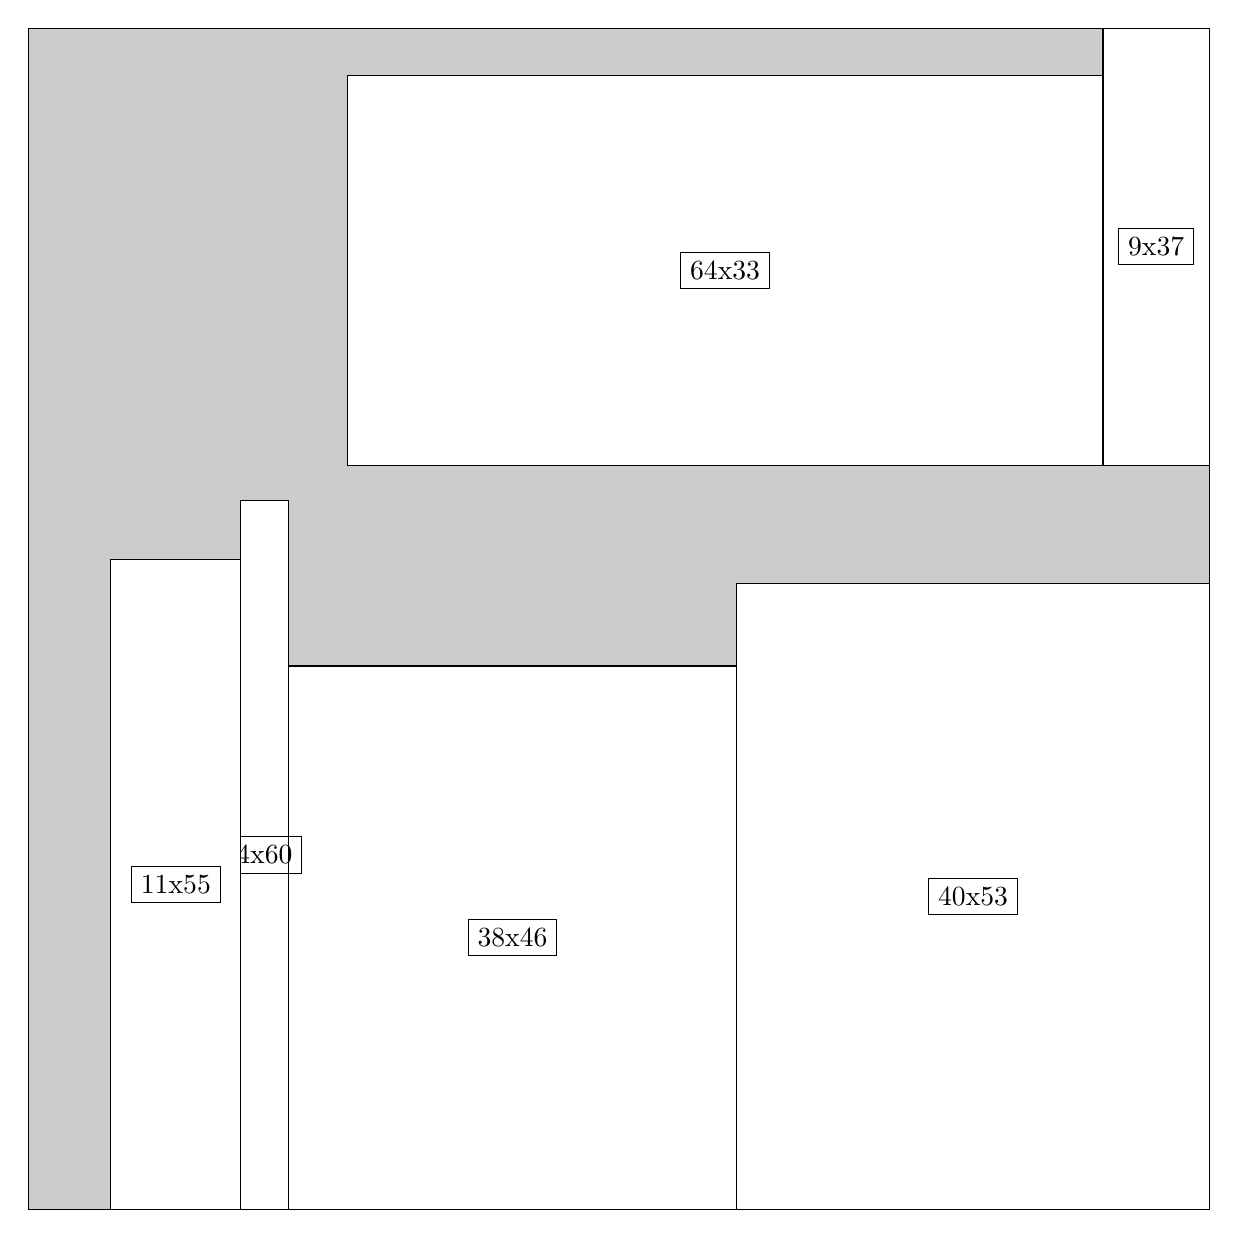
\begin{tikzpicture}[shorten >=1pt,scale=1.0,every node/.style={scale=1.0},->]
\tikzstyle{vertex}=[circle,fill=black!25,minimum size=14pt,inner sep=0pt]
\filldraw[fill=gray!40!white, draw=black] (0,0) rectangle (15.0,15.0);
\foreach \name/\x/\y/\w/\h in {40x53/9.0/0.0/6.0/7.949999999999999,38x46/3.3/0.0/5.7/6.8999999999999995,4x60/2.6999999999999997/0.0/0.6/9.0,11x55/1.05/0.0/1.65/8.25,9x37/13.65/9.45/1.3499999999999999/5.55,64x33/4.05/9.45/9.6/4.95}
\filldraw[fill=white!40!white, draw=black] (\x,\y) rectangle node[draw] (\name) {\name} ++(\w,\h);
\end{tikzpicture}


w =40 , h =53 , x =60 , y =0 , v =2120
\par
w =38 , h =46 , x =22 , y =0 , v =1748
\par
w =4 , h =60 , x =18 , y =0 , v =240
\par
w =11 , h =55 , x =7 , y =0 , v =605
\par
w =9 , h =37 , x =91 , y =63 , v =333
\par
w =64 , h =33 , x =27 , y =63 , v =2112
\par
\newpage


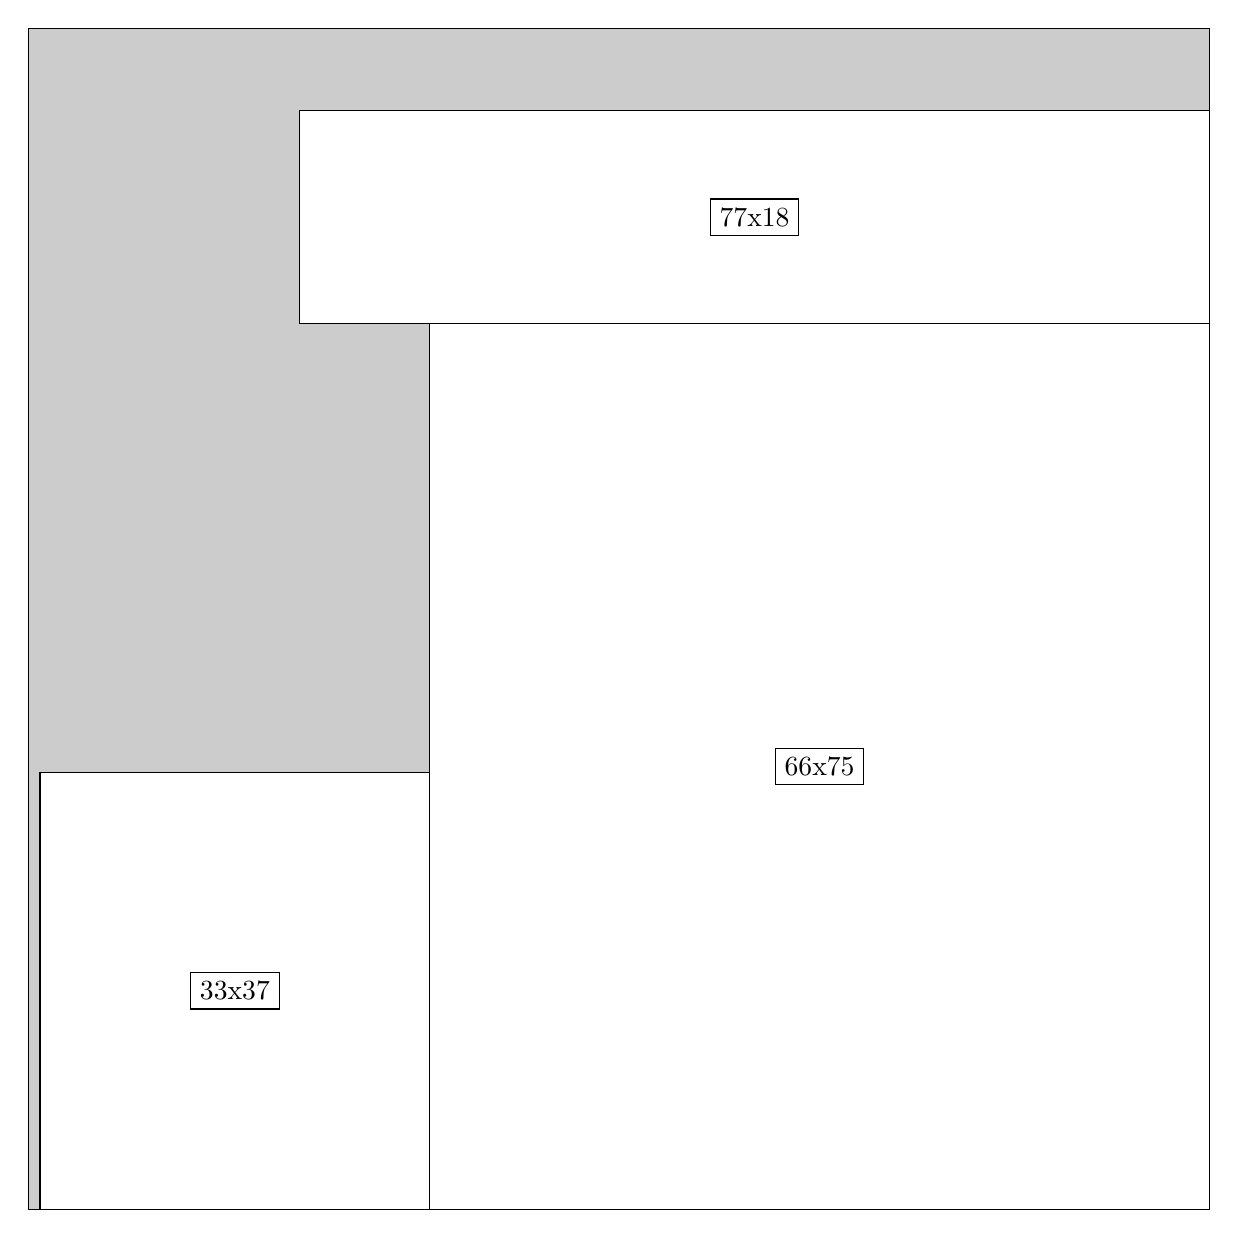
\begin{tikzpicture}[shorten >=1pt,scale=1.0,every node/.style={scale=1.0},->]
\tikzstyle{vertex}=[circle,fill=black!25,minimum size=14pt,inner sep=0pt]
\filldraw[fill=gray!40!white, draw=black] (0,0) rectangle (15.0,15.0);
\foreach \name/\x/\y/\w/\h in {66x75/5.1/0.0/9.9/11.25,33x37/0.15/0.0/4.95/5.55,77x18/3.4499999999999997/11.25/11.549999999999999/2.6999999999999997}
\filldraw[fill=white!40!white, draw=black] (\x,\y) rectangle node[draw] (\name) {\name} ++(\w,\h);
\end{tikzpicture}


w =66 , h =75 , x =34 , y =0 , v =4950
\par
w =33 , h =37 , x =1 , y =0 , v =1221
\par
w =77 , h =18 , x =23 , y =75 , v =1386
\par
\newpage


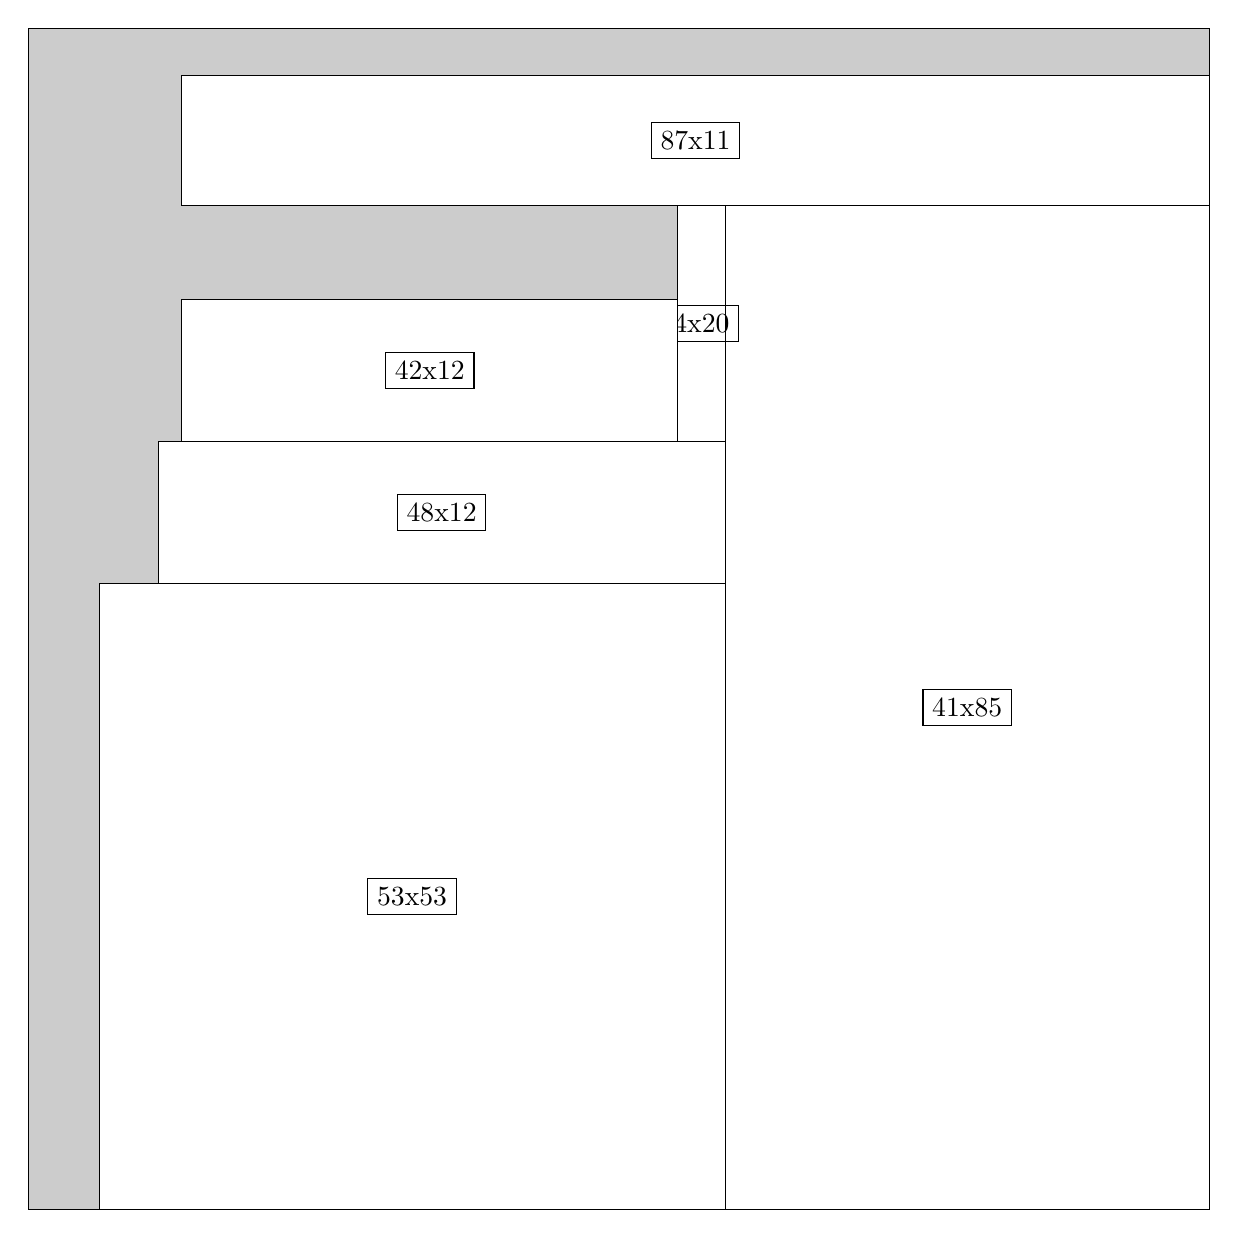
\begin{tikzpicture}[shorten >=1pt,scale=1.0,every node/.style={scale=1.0},->]
\tikzstyle{vertex}=[circle,fill=black!25,minimum size=14pt,inner sep=0pt]
\filldraw[fill=gray!40!white, draw=black] (0,0) rectangle (15.0,15.0);
\foreach \name/\x/\y/\w/\h in {41x85/8.85/0.0/6.1499999999999995/12.75,53x53/0.8999999999999999/0.0/7.949999999999999/7.949999999999999,48x12/1.65/7.949999999999999/7.199999999999999/1.7999999999999998,4x20/8.25/9.75/0.6/3.0,42x12/1.95/9.75/6.3/1.7999999999999998,87x11/1.95/12.75/13.049999999999999/1.65}
\filldraw[fill=white!40!white, draw=black] (\x,\y) rectangle node[draw] (\name) {\name} ++(\w,\h);
\end{tikzpicture}


w =41 , h =85 , x =59 , y =0 , v =3485
\par
w =53 , h =53 , x =6 , y =0 , v =2809
\par
w =48 , h =12 , x =11 , y =53 , v =576
\par
w =4 , h =20 , x =55 , y =65 , v =80
\par
w =42 , h =12 , x =13 , y =65 , v =504
\par
w =87 , h =11 , x =13 , y =85 , v =957
\par
\newpage


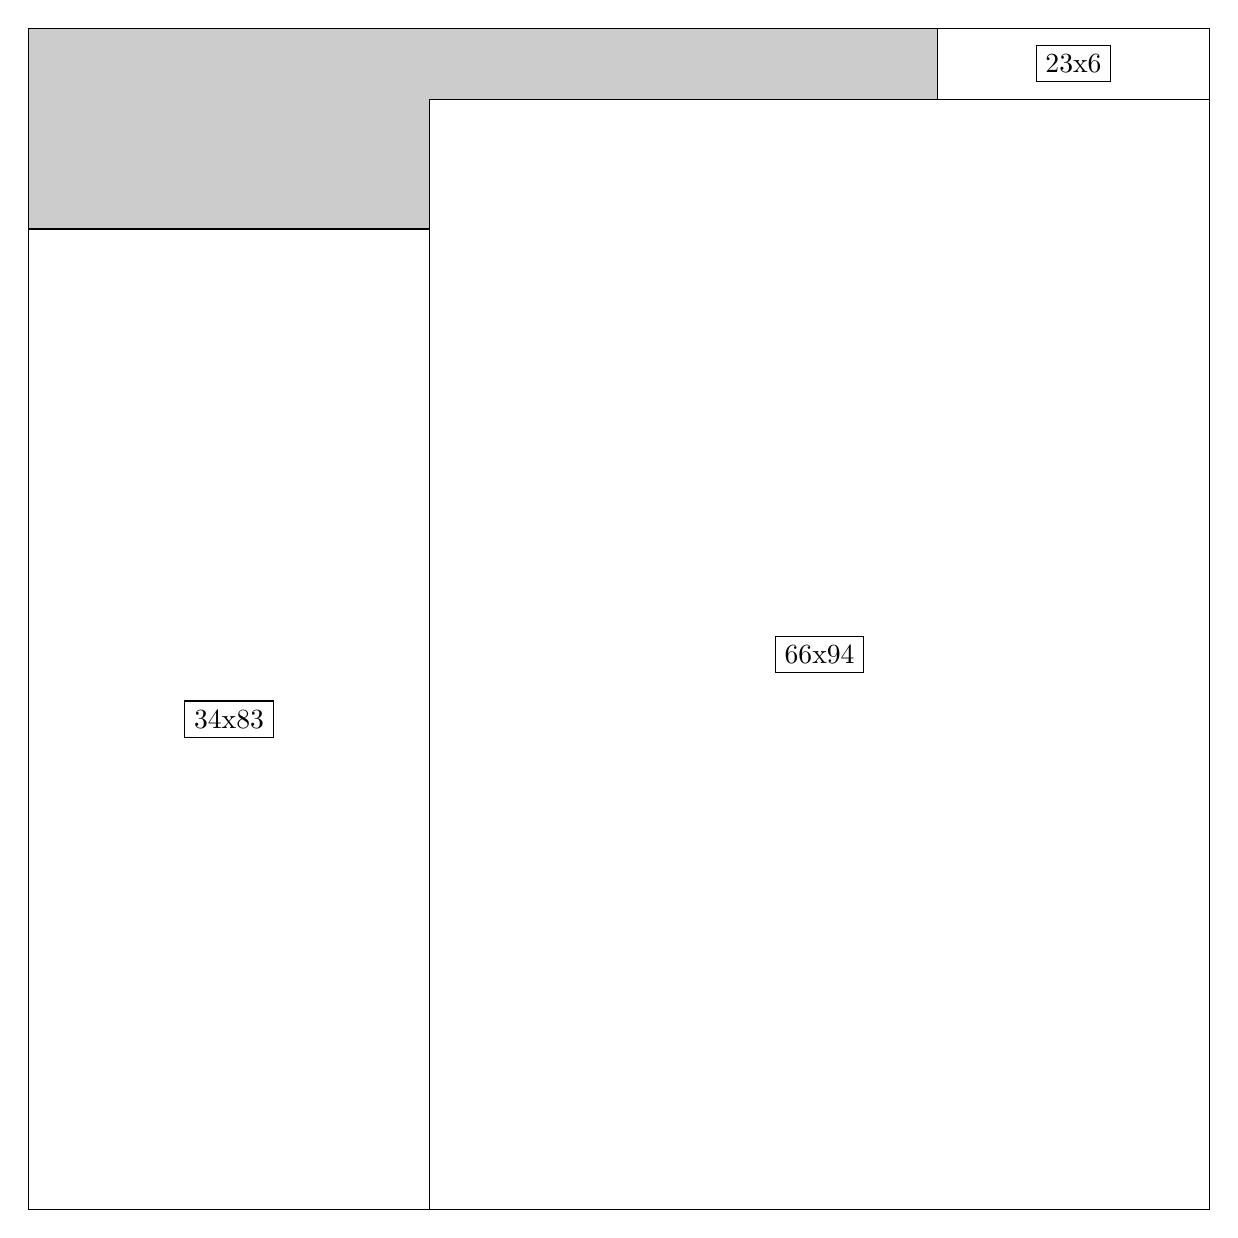
\begin{tikzpicture}[shorten >=1pt,scale=1.0,every node/.style={scale=1.0},->]
\tikzstyle{vertex}=[circle,fill=black!25,minimum size=14pt,inner sep=0pt]
\filldraw[fill=gray!40!white, draw=black] (0,0) rectangle (15.0,15.0);
\foreach \name/\x/\y/\w/\h in {66x94/5.1/0.0/9.9/14.1,34x83/0.0/0.0/5.1/12.45,23x6/11.549999999999999/14.1/3.4499999999999997/0.8999999999999999}
\filldraw[fill=white!40!white, draw=black] (\x,\y) rectangle node[draw] (\name) {\name} ++(\w,\h);
\end{tikzpicture}


w =66 , h =94 , x =34 , y =0 , v =6204
\par
w =34 , h =83 , x =0 , y =0 , v =2822
\par
w =23 , h =6 , x =77 , y =94 , v =138
\par
\newpage


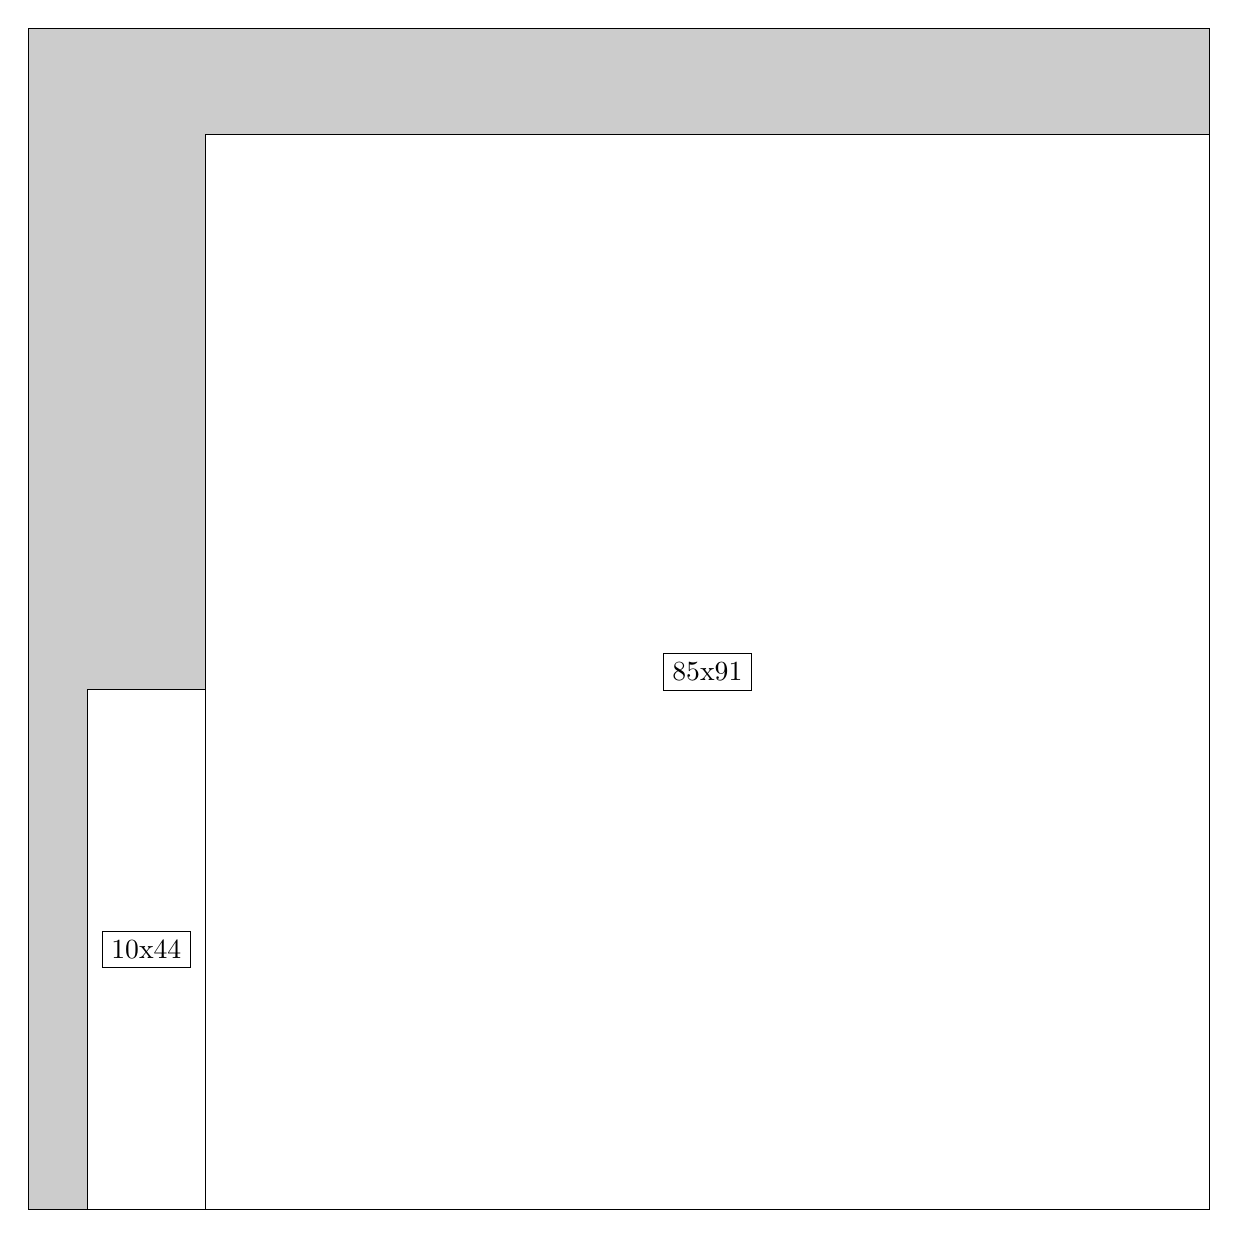
\begin{tikzpicture}[shorten >=1pt,scale=1.0,every node/.style={scale=1.0},->]
\tikzstyle{vertex}=[circle,fill=black!25,minimum size=14pt,inner sep=0pt]
\filldraw[fill=gray!40!white, draw=black] (0,0) rectangle (15.0,15.0);
\foreach \name/\x/\y/\w/\h in {85x91/2.25/0.0/12.75/13.65,10x44/0.75/0.0/1.5/6.6}
\filldraw[fill=white!40!white, draw=black] (\x,\y) rectangle node[draw] (\name) {\name} ++(\w,\h);
\end{tikzpicture}


w =85 , h =91 , x =15 , y =0 , v =7735
\par
w =10 , h =44 , x =5 , y =0 , v =440
\par
\newpage


\end{document}